\section{Systemet}
Her vil systemet blive gennemgået og der vil blive gået i dybden med nogle kodeeksempler, for at give et bedre overblik over hvordan systemet virker og er sat sammen.
De eksempler vi gennemgår er dem der har mest betydning for hvordan systemet virker og er kernefunktionalitet.
\subsection{getStatisticsData}
\begin{lstlisting}[caption={getStatisticsData}, language={JavaScript}, label={lst:StatisticsControllerData}]
ctrl.getStatisticsData = function(statisticIndex, statisticType) {
    statsIndexId = statisticIndex;
    statsTypeId = statisticType;

    showStatistics.get({
        statsIndex : statsIndexId,
        statsType : statsTypeId
        })
        .$promise.then(function(data) {
            ctrl.fetchedData = data.hits.hits[0];
            filterData(ctrl.fetchedData._source.type);

            var dataObject = {
                'index' : ctrl.fetchedData._index,
                'type' : ctrl.fetchedData._type,
                'data' : ctrl.filteredValue,
                'checked' : false
            };

            var duplicate = false;

            for(i = 0; i < ctrl.chartData.length; i++) {
                // check for duplicates in chartData list
                if(dataObject.type == ctrl.chartData[i].type) {
                    duplicate = true;
                }
            }

            if(!duplicate) {
                ctrl.chartData.push(dataObject);
            }
        });
};
\end{lstlisting}
i kodeeksempel~\ref{lst:StatisticsControllerData}, hentes der statistik data ud fra et valgt API.
Vi benytter os af et promise som gør, at vi kan håndtere forskellige resultater, alt efter om det lykkedes at hente noget data, fra ElasticSeach, eller ej.
\\\\
Måden vi implementerede det på i vores view, ses på figur~\ref{fig:getStatisticsData} for at gøre det nemt og overskueligt for brugeren,
når de skal vælge statistic data.
Den henter index og type ud fra vores MySQL database.
\begin{figure}[H]
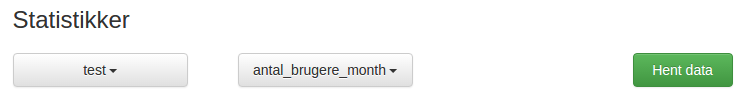
\includegraphics[scale=0.5]{getStatisticsData}
\caption{getStatisticData view}
\label{fig:getStatisticsData}
\end{figure}
\subsubsection{Reflektion over getStatisticsData}
Vi udnytter ikke et angular promise ordentligt og skulle have indlagt noget fejlhåndtering, hvis der ikke kom noget data fra API'et,
altså hvis promiset blev rejected.
Derudover har Angular gjort det rigtig nemt for os at arbejde med RESTful API's, pga.\ af ngResource~\footnote{https://docs.angularjs.org/api/ngResource}.
\subsection{drawChart}
\begin{lstlisting}[caption={drawChart}, language={JavaScript}, label={lst:StatisticsControllerDraw}]
ctrl.drawChart = function(chartType, data, title) {
    chartObject = {};
    chartObject.type = chartType;
    chartObject.data = formatChartData(data);
    chartObject.options = {
        displayExactValues: true,
        width: 600,
        height: 600,
        is3D: true,
        title: title
    };
    ctrl.chart = chartObject;
};

formatChartData = function(data) {
    chartObjectData = [
        ['ChartData', 'data']
    ];

    for(i = 0; i < ctrl.chartData.length; i++) {
        currentDataObject = ctrl.chartData[i];

        if(currentDataObject.checked) {
            chartObjectData.push([
                    currentDataObject.data[0],
                    currentDataObject.data[1]
            ]);
        }
    }
    return chartObjectData;
};
\end{lstlisting}
I kodeeksempel~\ref{lst:StatisticsControllerDraw} bruges den valgte data, vi har fra figur~\ref{fig:getStatisticsData}.
Vi benytter os af \hyperlink{GoogleChartAPI}{Google Chart API}, hvor vi sætter de nødvendige properties for at lave et diagram.
Hvis vi kigger fremad kunne vi have lavet det, så man selv kunne bestemme størrelsen på diagrammet. Vi valgte løsningen med faste værdier, da det var vigtigt for os, at have noget funktionelt
og ligetil.
\\\\
Koden er delt op i to funktioner, hhv.\ formatChartData og drawChart, da det giver et bedre overblik over hele controlleren.
I figur~\ref{fig:drawChart} kan man se hvordan de to funktioner er implementeret i vores view.
\begin{figure}[H]
\centering
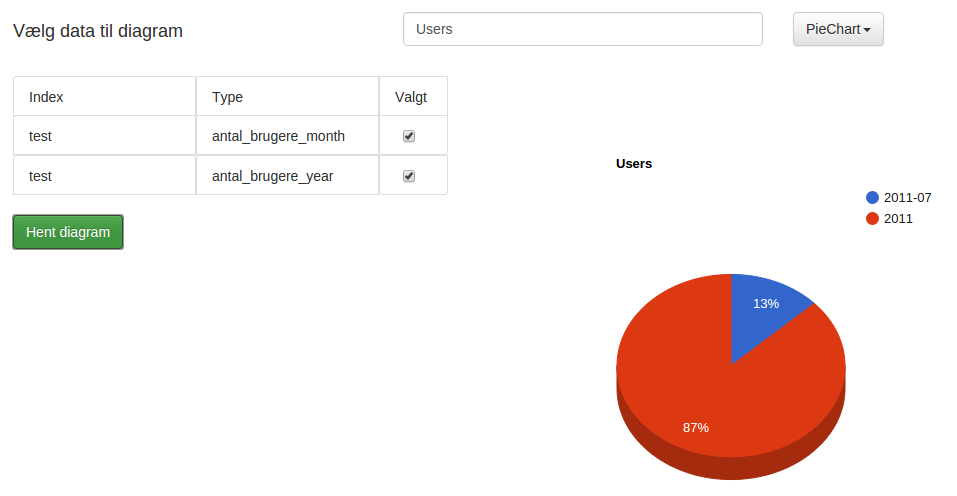
\includegraphics[scale=0.4]{drawChart}
\caption{drawChart view}
\label{fig:drawChart}
\end{figure}
\subsection{pullData}
\begin{lstlisting}[caption={pullData}, language={JavaScript}, label={lst:PullControllerPullData}]
ctrl.pullData = function(index, type, api) {
    var apiData = null;
    testRemoteApi.get({ apiUrl : api }).$promise.then(function(data) {
        apiData = data;

        if (data.error) {
            ctrl.error = data.error;
            $timeout(function() {
                ctrl.error = '';
            }, 3000);
        } else {
            var apiES = {
                'index': index,
                'type': type,
                'body': { type: apiData }
            };

            // Index the api data in ElasticSearch
            elasticIndex.save(apiES).$promise.then(function() {
                var apiRemote = {
                    'index' : index,
                    'type' : type,
                    'url' : api
                };

                // Save the api data in sql db
                saveRemoteApi.save(apiRemote).$promise.then(function() {
                    ctrl.success = api + ' blev gemt';
                    $timeout(function() {
                        ctrl.success = '';
                    }, 3000);
    });
}
\end{lstlisting}
I kodeeksempel~\ref{lst:PullControllerPullData} er metoden beskåret, så det kun er kernefunktionaliteten der er tilbage i den.
Det er funktionen der håndterer de API'er vi skal kunne hente data fra, det er også den funktion der sørger for at de bliver gemt 
i MySQL databasen, så de kan bruges af getStatisticsData. Koden sørger for at indexere den data fra API'et i vores ElasticSearch
database.
I figur~\ref{fig:pullData} vises hvordan vi har implementeret pullData. Som det er nu, er \textbf{Validér API Endpoint} knappen altid deaktiveret. 
Det er planen at i fremtiden, vil man kunne validere at det er et valid endpoint, med valid data.
\\\\
Derudover ville det nok have været smartest, at dele denne funktion op i mindre funktioner. Så den ikke både håndterede at kalde API'et der gemmer i MySQL databasen,
og det API der indekserer i ElasticSearch databasen.
\begin{figure}[H]
     \centering
     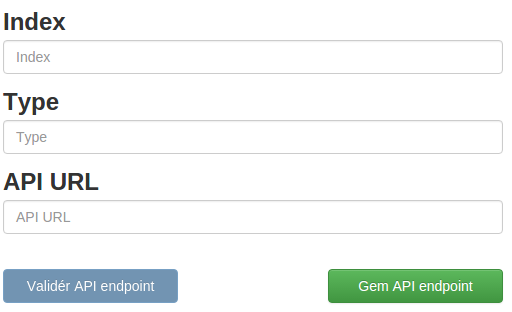
\includegraphics[scale=0.5]{pullData}
     \caption{pullData view}
     \label{fig:pullData}
\end{figure}
